\documentclass{article}[18pt]
\ProvidesPackage{format}
%Page setup
\usepackage[utf8]{inputenc}
\usepackage[margin=0.7in]{geometry}
\usepackage{parselines} 
\usepackage[english]{babel}
\usepackage{fancyhdr}
\usepackage{titlesec}
\hyphenpenalty=10000

\pagestyle{fancy}
\fancyhf{}
\rhead{Sam Robbins}
\rfoot{Page \thepage}

%Characters
\usepackage{amsmath}
\usepackage{amssymb}
\usepackage{gensymb}
\newcommand{\R}{\mathbb{R}}

%Diagrams
\usepackage{pgfplots}
\usepackage{graphicx}
\usepackage{tabularx}
\usepackage{relsize}
\pgfplotsset{width=10cm,compat=1.9}
\usepackage{float}

%Length Setting
\titlespacing\section{0pt}{14pt plus 4pt minus 2pt}{0pt plus 2pt minus 2pt}
\newlength\tindent
\setlength{\tindent}{\parindent}
\setlength{\parindent}{0pt}
\renewcommand{\indent}{\hspace*{\tindent}}

%Programming Font
\usepackage{courier}
\usepackage{listings}
\usepackage{pxfonts}

%Lists
\usepackage{enumerate}
\usepackage{enumitem}

% Networks Macro
\usepackage{tikz}


% Commands for files converted using pandoc
\providecommand{\tightlist}{%
	\setlength{\itemsep}{0pt}\setlength{\parskip}{0pt}}
\usepackage{hyperref}

% Get nice commands for floor and ceil
\usepackage{mathtools}
\DeclarePairedDelimiter{\ceil}{\lceil}{\rceil}
\DeclarePairedDelimiter{\floor}{\lfloor}{\rfloor}

% Allow itemize to go up to 20 levels deep (just change the number if you need more you madman)
\usepackage{enumitem}
\setlistdepth{20}
\renewlist{itemize}{itemize}{20}

% initially, use dots for all levels
\setlist[itemize]{label=$\cdot$}

% customize the first 3 levels
\setlist[itemize,1]{label=\textbullet}
\setlist[itemize,2]{label=--}
\setlist[itemize,3]{label=*}

% Definition and Important Stuff
% Important stuff
\usepackage[framemethod=TikZ]{mdframed}

\newcounter{theo}[section]\setcounter{theo}{0}
\renewcommand{\thetheo}{\arabic{section}.\arabic{theo}}
\newenvironment{important}[1][]{%
	\refstepcounter{theo}%
	\ifstrempty{#1}%
	{\mdfsetup{%
			frametitle={%
				\tikz[baseline=(current bounding box.east),outer sep=0pt]
				\node[anchor=east,rectangle,fill=red!50]
				{\strut Important};}}
	}%
	{\mdfsetup{%
			frametitle={%
				\tikz[baseline=(current bounding box.east),outer sep=0pt]
				\node[anchor=east,rectangle,fill=red!50]
				{\strut Important:~#1};}}%
	}%
	\mdfsetup{innertopmargin=10pt,linecolor=red!50,%
		linewidth=2pt,topline=true,%
		frametitleaboveskip=\dimexpr-\ht\strutbox\relax
	}
	\begin{mdframed}[]\relax%
		\centering
		}{\end{mdframed}}



\newcounter{lem}[section]\setcounter{lem}{0}
\renewcommand{\thelem}{\arabic{section}.\arabic{lem}}
\newenvironment{defin}[1][]{%
	\refstepcounter{lem}%
	\ifstrempty{#1}%
	{\mdfsetup{%
			frametitle={%
				\tikz[baseline=(current bounding box.east),outer sep=0pt]
				\node[anchor=east,rectangle,fill=blue!20]
				{\strut Definition};}}
	}%
	{\mdfsetup{%
			frametitle={%
				\tikz[baseline=(current bounding box.east),outer sep=0pt]
				\node[anchor=east,rectangle,fill=blue!20]
				{\strut Definition:~#1};}}%
	}%
	\mdfsetup{innertopmargin=10pt,linecolor=blue!20,%
		linewidth=2pt,topline=true,%
		frametitleaboveskip=\dimexpr-\ht\strutbox\relax
	}
	\begin{mdframed}[]\relax%
		\centering
		}{\end{mdframed}}
\lhead{Networks and Systems - Networking}
\usepackage{minted}

\begin{document}
\begin{center}
\underline{\huge Application Layer}
\end{center}
\section{Application Layer}
Network Architecture:
\begin{itemize}
	\item Client-server architecture
	\item P2P Architecture
\end{itemize}
Processes and Socket programming
\begin{itemize}
	\item TCP
	\item UDP
\end{itemize}
\section{Creating a network app}
Write programs that:
\begin{itemize}
	\item Run on (different) end systems
	\item Communicate over network
\end{itemize}
No need to write software for network-core devices
\begin{itemize}
	\item Network-core devices do not run user applications
	\item Applications on end systems allow for rapid app development, propagation 
\end{itemize}
\section{Application Architectures}
\subsection{Client-Server Architecture}
Server:
\begin{itemize}
	\item Always-on host
	\item Fixed (static) IP address
	\item Data centres for scaling
\end{itemize}
Clients
\begin{itemize}
	\item Communicate with server
	\item May be intermittently connected
	\item May have dynamic IP addresses
	\item Do not communicate directly with each other
\end{itemize}
\subsection{P2P Architecture}
\begin{itemize}
	\item No always on server
	\item Arbitrary end systems directly communicate
	\item Peers request service from other peers, provide service in return to other peers
	\item Self scalability - new peers bring service capacity, as well as new service demands
	\item Peers are intermittently connected and change IP addresses
\end{itemize}
\subsection{Hybrid}
\begin{itemize}
	\item Often there is a hybrid architecture, an example of this might be video calling, the initial connection and authentication might be handled by a server, but the actual video will be sent via P2P
\end{itemize}
\section{Processes communicating}
\begin{defin}[Process]
A program running within a host
\end{defin}
\begin{defin}[Socket]
A software mechanism that allows a process to create and send messages into, and receive messages from the network
\end{defin}
\begin{itemize}
	\item Within same host, two processes communicate using inter-process communication (defined by OS)
	\item Processes in different hosts communicate by exchanging messages
	\item A process is analogous to a house, and its socket is analogous to its door
	\item Interface between application layer and transport layer
\end{itemize}
\section{Sockets}
\begin{itemize}
	\item Process sends/receives messages to/from its socket
	\item A socket shoves message out of the door
	\item Sending process relies on transport infrastructure on the other side of the door to deliver message to a socket at the receiving process
\end{itemize}
\begin{center}
	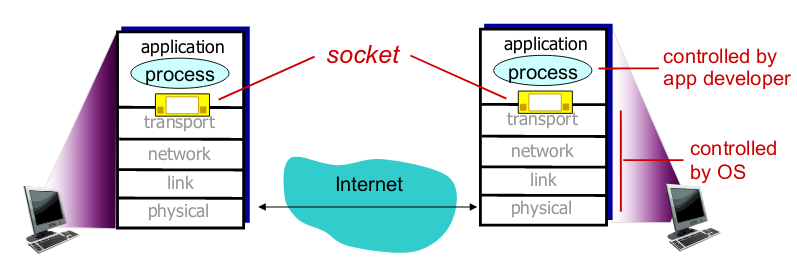
\includegraphics[scale=0.7]{sockets}
\end{center}
\section{What transport service does an app need?}
Data integrity
\begin{itemize}
	\item Some apps (e.g. file transfer, web transactions) require 100\% reliable data transfer
	\item Other apps (e.g. audio) can tolerate some loss
\end{itemize}
Security:
\begin{itemize}
	\item Encryption, data integrity, ...
\end{itemize}
Timing:
\begin{itemize}
	\item Some apps (e.g. internet telephony, interactive games) require low delay to be "effective"
\end{itemize}
\section{Internet Transport Protocols Service}

TCP Service:
\begin{itemize}
	\item \textbf{Connection-Oriented}: Setup required between client and server process
	\item \textbf{Reliable transport} between sending and receiving processes
	\item \textbf{Flow control}: Sender won't overwhelm receiver
	\item \textbf{Full-duplex connection}: Connection can send messages to each other at the same time
\end{itemize}


UDP service:
\begin{itemize}
	\item \textbf{Unreliable data transfer} between sending and receiving processes
	\item \textbf{Does not provide} reliability, flow control, timing, security or connection setup
\end{itemize}

\section{App-layer protocol defines}
\begin{itemize}
	\item Types of messages exchanged - E.g. request, response
	\item Message syntax - What fields in messages \& how fields are delineated
	\item Message semantics - Meaning of information in fields
	\item Rules for when and how processes send \& respond to messages
\end{itemize}
\begin{defin}[Open protocols]
Defined in Request For Comments (RFC) Allow for interoperability e.g. HTTP, SMTP 
\end{defin}
\section{HTTP Overview}
\begin{defin}[HTTP (Hypertext transfer protocol)]
Web's application layer protocol
\end{defin}
HTTP uses TCP:
\begin{itemize}
	\item Client initiates TCP connection (creates socket) to server, port 80
	\item Server accepts TCP connection from client
	\item HTTP messages (application - layer protocol messages) exchanged between browser (HTTP client) and web server (HTTP server)
	\item TCP connection closed
\end{itemize}
\begin{important}[HTTP]
HTTP is stateless - server maintains no information about past client requests
\end{important}
\begin{defin}[Client/Server Model]
\textbf{Client} - Browser that requests, receives, (using HTTP Protocol) and "displays" web objects\\
\textbf{Server}: Web server sends (using HTTP protocol) objects in response to requests 
\end{defin}
\section{HTTP Connections}
Non persistent HTTP
\begin{itemize}
	\item At most one object sent over TCP connection, connection then closed
\end{itemize}
Persistent HTTP
\begin{itemize}
	\item Multiple objects can be sent over single TCP connection, between client, server
\end{itemize}
\subsection{Non-persistent HTTP}
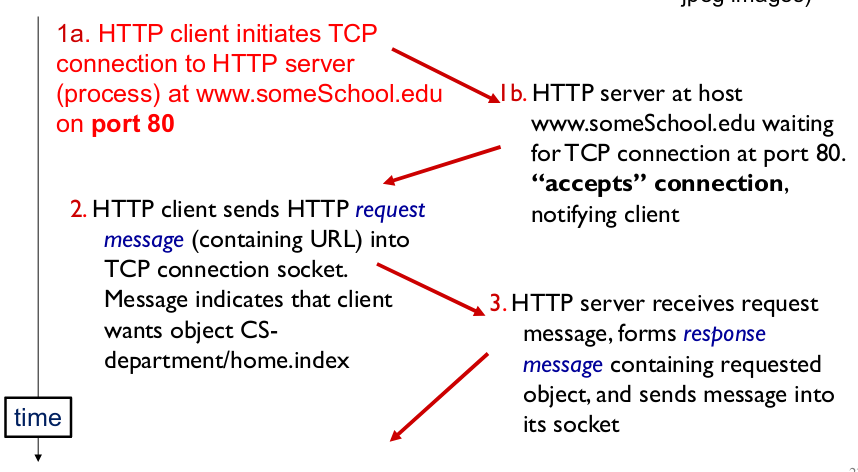
\includegraphics[scale=0.7]{HTTP}\\
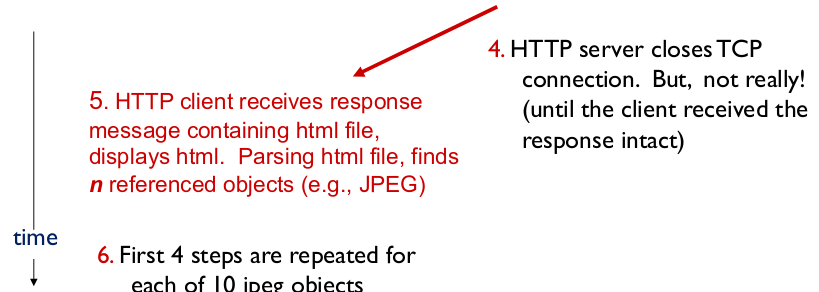
\includegraphics[scale=0.7]{HTTP2}
\subsubsection{Response Time}
\begin{defin}[RTT (Round trip time)]
The for a small packet to travel from client to server and back
\end{defin}
HTTP Response time:
\begin{itemize}
	\item One RTT to initiate TCP connection
	\item One RTT for HTTP request and first few bytes of HTTP response to return
	\item File transmission time
	\item Non-persistent HTTP response time = 2RTT + file transmission time\\
	Incurred for each file
\end{itemize}
\begin{center}
	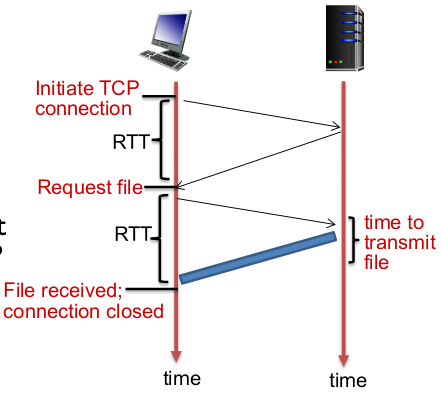
\includegraphics[scale=0.7]{RTT}
\end{center}
\subsection{Persistent HTTP}
\begin{itemize}
	\item Server leaves connection open after sending response
	\item Subsequent HTTP messages between same client/server sent over open connection
	\item Client sends requests as soon as it encounters a referenced object
	\item Takes as little as one RTT + file transmission time total
	\begin{itemize}
		\item Assuming connections to server already established
		\item Assuming all files requested in parallel
	\end{itemize}
\end{itemize}
\section{Socket Programming}
\textbf{Goal}: learn how to build client/server applications that communicate using sockets\\
\textbf{Socket}: door between application process and end-end-transport protocol\\
\\
Two socket types for two transport services:
\begin{itemize}
	\item UDP: unreliable datagram
	\item TCP: reliable, byte stream-oriented
\end{itemize}
Application example:
\begin{enumerate}
	\item Client reads a line of characters (data) from its keyboard and sends data to server
	\item Server receives the data and converts characters to uppercase
	\item Server sends modified data to client
	\item Client receives modified data and displays line on the screen
\end{enumerate}
\subsection{Socket programming with UDP}
\begin{itemize}
	\item UDP: no "connection" between client \& server
	\item No handshaking before sending data
	\item Sender explicitly attaches IP destination address and port \# to each packet
	\item Receiver extracts sender IP address and port\# from received packet
	\item UDP: transmitted data may be lost or received out-of-order
	\item Application viewpoint:
	\item UDP provides unreliable transfer of groups of bytes ("datagrams") between client and server
\end{itemize}
\subsubsection{Client/server socket interaction: UDP}
\begin{center}
	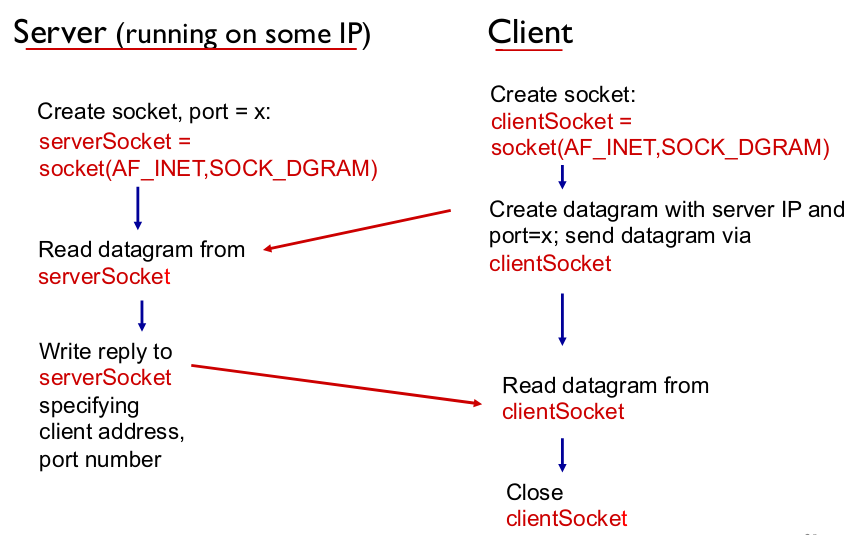
\includegraphics[scale=0.7]{UDP}
\end{center}
\subsubsection{Example app: UDP client}
\begin{minted}{python}
# include python's socket library
from socket import *
# If server IP is empty then local system
serverName =''
# choose an unreserved port
serverPort=12000
# create UDP socket for server
clientSocket=socket(AF_INET, SOCK_DGRAM)
# get user keyboard input
message=input('Input lowercase sentence: ')
# Attach server name, port to message; send into socket
clientSocket.sendto(message.encode(),(serverName,ServerPort))
# Read reply characters from socket into string
modifiedMessage, serverAddress = clientSocket.recvfrom(2048)
# Print out recived string and close socket
print(modifiedMessage.decode())
clientSocket.close()
\end{minted}
\subsubsection{Example app: UDP server}
\begin{minted}{python}
from socket import *
serverPort = 12000
# Create UDP socket
serverSocket = socket(AF_INET, SOCK_DGRAM)
# Bind socket to local port number 12000
serverSocket.bind(('', serverPort))
print('The serve is ready to receive')
# while True
	# Read from UDP socket into message, getting client's address (client IP and port)
	message, clientAddress = serverSocket.recvfrom(2048)
	# Send upper case string back to this client
	modifiedMessage = message.decode().upper()
	serverSocket.sendto(modifiedMessage.encode)
\end{minted}
\section{Socket Programming with TCP}
\begin{itemize}
	\item Client must contact server
	\item Server process must first be running
	\item Server must have created socket that welcomes client's contact
	\item Client contacts server by
	\begin{itemize}
		\item Creating TCP socket, specifying IP address, port number of server process
	\end{itemize}
	\item When client establishes socket: client TCP establishes connection to server TCP
	\item When contacted by the client:
	\begin{itemize}
		\item Server TCP create new socket for server process to communicate with that particular client
	\end{itemize}
	\item Allows server to talk with multiple clients
	\item Source port numbers used to distinguish clients
\end{itemize}
Application viewpoint:
\begin{itemize}
	\item TCP provides reliable, in-order byte-stream transfer ("pipe") between client and server
\end{itemize}
\subsection{Client/server socket interaction: TCP}
\begin{center}
	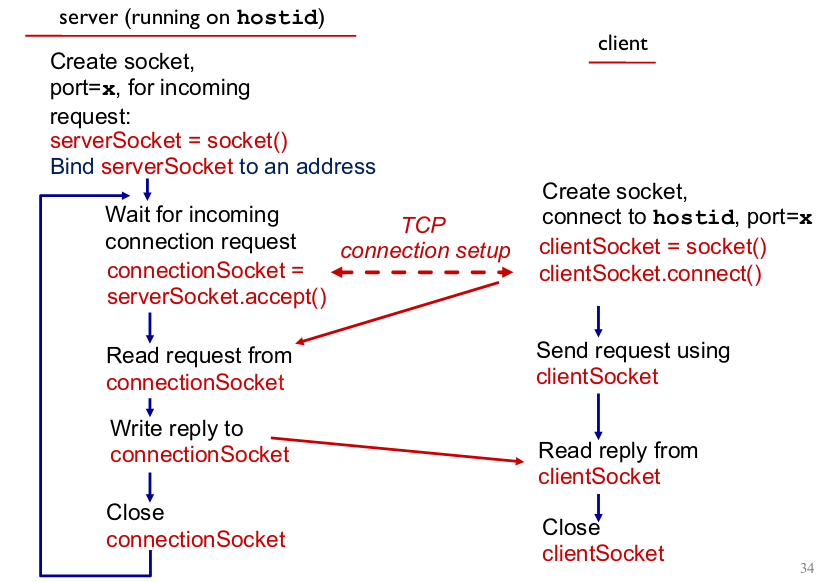
\includegraphics[scale=0.5]{TCP}
\end{center}
\subsection{Example app: TCP Client}
\begin{minted}{python}
from socket import *
serverName=''
serverPort=12000
clientSocket=socket(AF_INET,SOCK_STREAM)
clientSocket.connect((serverName, serverPort))
sentence=input('Input lowercase sentence: ')
clientSocket.send(sentence.encode())
modifiedSentence=clientSocket.recv(1024)
print('From Server: ', modifiedSentence.decode())
clientSocket.close()
\end{minted}

\subsection{Example app: TCP server}
\begin{minted}{python}
from socket import *
serverPort=12000
# Create TCP welcoming socket
serverSocket = socket(AF_INET,SOCK_STREAM)
serverSocket.bind(('',serverPort))
# Server begins listening for incoming TCP requests
serverSocket.listen(1)
print('The server is ready to revieve')
while True:
	# Server waits on accept() for incoming requests, new socket created on return
	connectionSocket, addr=serverSocket.accept()
	# Read bytes from socket (not address as in UDP)
	sentence=connectionSocket.recv(1024).decode()
	capsSentence=sentence.upper()
	connectionSocket.send(capsSentence)
	# Close connection to this client (but not welcoming socket)
	connectionSocket.close()
\end{minted}


\end{document}